\documentclass{standalone}
\usepackage{tikz}
\usepackage{xcolor}
\usetikzlibrary{patterns, positioning}

    \usetikzlibrary{calc}
    \usepackage{relsize}
    \tikzset{fontscale/.style = {font=\relsize{#1}}}
\begin{document}
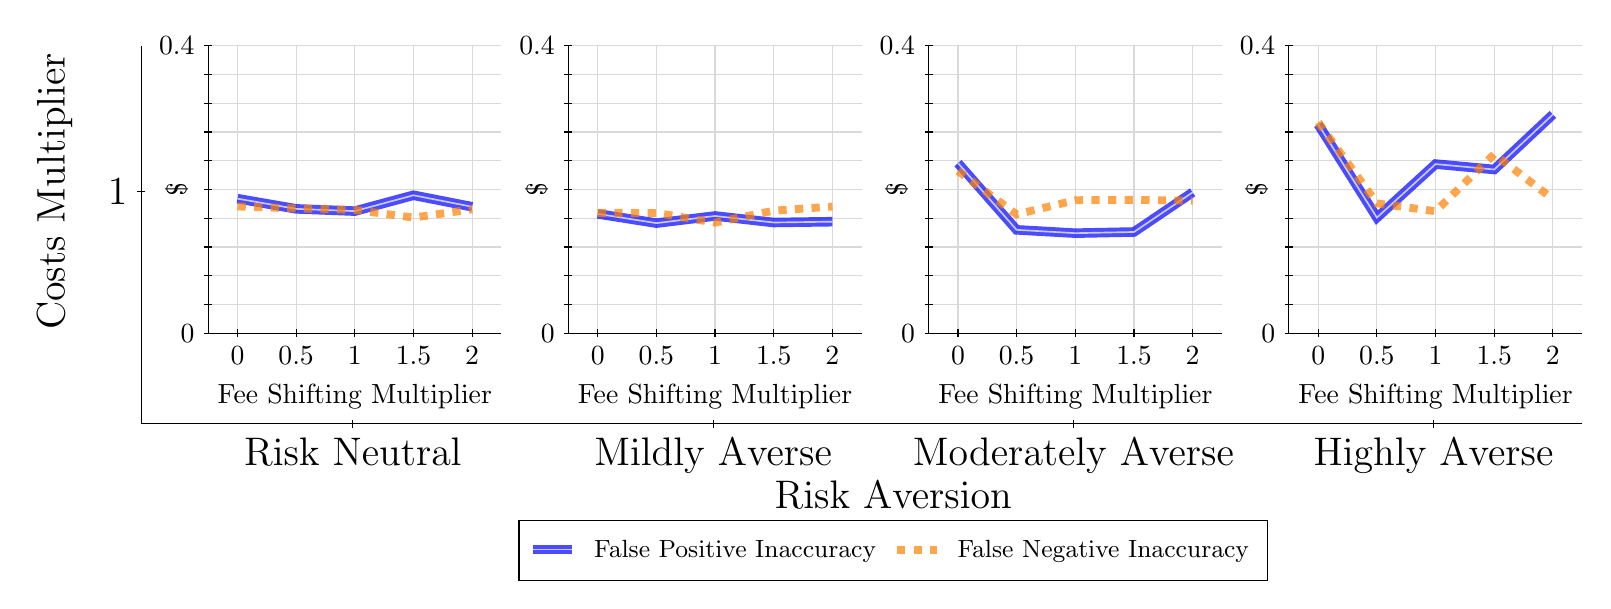
\begin{tikzpicture}
\draw[black] (1.7,1.5) -- (1.7,6.3);
\node[rotate=90, fontscale=2, anchor=center] at (0.6, 4.45) {Costs Multiplier};
\draw[black] (1.65,4.45) -- (1.75,4.45);
\node[fontscale=2, anchor=east] at (1.65, 4.45) {1};

\draw[black] (1.7,1.5) -- (20,1.5);
\node[fontscale=2, anchor=center] at (11.25, 0.6) {Risk Aversion};
\draw[black] (4.3875,1.45) -- (4.3875,1.55);
\node[fontscale=2, anchor=north] at (4.3875, 1.45) {Risk Neutral};
\draw[black] (8.9625,1.45) -- (8.9625,1.55);
\node[fontscale=2, anchor=north] at (8.9625, 1.45) {Mildly Averse};
\draw[black] (13.538,1.45) -- (13.538,1.55);
\node[fontscale=2, anchor=north] at (13.538, 1.45) {Moderately Averse};
\draw[black] (18.112,1.45) -- (18.112,1.55);
\node[fontscale=2, anchor=north] at (18.112, 1.45) {Highly Averse};


\draw[gray!30] (2.55,2.65) -- (6.275,2.65);
\draw[gray!30] (2.55,3.015) -- (6.275,3.015);
\draw[gray!30] (2.55,3.38) -- (6.275,3.38);
\draw[gray!30] (2.55,3.745) -- (6.275,3.745);
\draw[gray!30] (2.55,4.11) -- (6.275,4.11);
\draw[gray!30] (2.55,4.475) -- (6.275,4.475);
\draw[gray!30] (2.55,4.84) -- (6.275,4.84);
\draw[gray!30] (2.55,5.205) -- (6.275,5.205);
\draw[gray!30] (2.55,5.57) -- (6.275,5.57);
\draw[gray!30] (2.55,5.935) -- (6.275,5.935);
\draw[gray!30] (2.55,6.3) -- (6.275,6.3);
\draw[gray!30] (2.9225,2.65) -- (2.9225,6.3);
\draw[gray!30] (3.6675,2.65) -- (3.6675,6.3);
\draw[gray!30] (4.4125,2.65) -- (4.4125,6.3);
\draw[gray!30] (5.1575,2.65) -- (5.1575,6.3);
\draw[gray!30] (5.9025,2.65) -- (5.9025,6.3);
\draw[black] (2.55,2.65) -- (2.55,6.3);
\node[rotate=90, fontscale=0.7, anchor=center] at (2.15, 4.475) {\$};
\draw[black] (2.5,2.65) -- (2.6,2.65);
\node[fontscale=0.7, anchor=east] at (2.5, 2.65) {0};
\draw[black] (2.5,3.015) -- (2.6,3.015);
\node[fontscale=0.7, anchor=east] at (2.5, 3.015) { };
\draw[black] (2.5,3.38) -- (2.6,3.38);
\node[fontscale=0.7, anchor=east] at (2.5, 3.38) { };
\draw[black] (2.5,3.745) -- (2.6,3.745);
\node[fontscale=0.7, anchor=east] at (2.5, 3.745) { };
\draw[black] (2.5,4.11) -- (2.6,4.11);
\node[fontscale=0.7, anchor=east] at (2.5, 4.11) { };
\draw[black] (2.5,4.475) -- (2.6,4.475);
\node[fontscale=0.7, anchor=east] at (2.5, 4.475) { };
\draw[black] (2.5,4.84) -- (2.6,4.84);
\node[fontscale=0.7, anchor=east] at (2.5, 4.84) { };
\draw[black] (2.5,5.205) -- (2.6,5.205);
\node[fontscale=0.7, anchor=east] at (2.5, 5.205) { };
\draw[black] (2.5,5.57) -- (2.6,5.57);
\node[fontscale=0.7, anchor=east] at (2.5, 5.57) { };
\draw[black] (2.5,5.935) -- (2.6,5.935);
\node[fontscale=0.7, anchor=east] at (2.5, 5.935) { };
\draw[black] (2.5,6.3) -- (2.6,6.3);
\node[fontscale=0.7, anchor=east] at (2.5, 6.3) {0.4};

\draw[black] (2.55,2.65) -- (6.275,2.65);
\node[fontscale=0.7, anchor=center] at (4.4125, 1.85) {Fee Shifting Multiplier};
\draw[black] (2.9225,2.6) -- (2.9225,2.7);
\node[fontscale=0.7, anchor=north] at (2.9225, 2.6) {0};
\draw[black] (3.6675,2.6) -- (3.6675,2.7);
\node[fontscale=0.7, anchor=north] at (3.6675, 2.6) {0.5};
\draw[black] (4.4125,2.6) -- (4.4125,2.7);
\node[fontscale=0.7, anchor=north] at (4.4125, 2.6) {1};
\draw[black] (5.1575,2.6) -- (5.1575,2.7);
\node[fontscale=0.7, anchor=north] at (5.1575, 2.6) {1.5};
\draw[black] (5.9025,2.6) -- (5.9025,2.7);
\node[fontscale=0.7, anchor=north] at (5.9025, 2.6) {2};

\draw[blue, opacity=0.70, line width=0.5mm, double] (2.9225,4.359) -- (3.6675,4.2291) -- (4.4125,4.2006) -- (5.1575,4.402) -- (5.9025,4.2558);
\draw[orange, opacity=0.70, line width=1mm, dashed] (2.9225,4.2595) -- (3.6675,4.2348) -- (4.4125,4.2165) -- (5.1575,4.1182) -- (5.9025,4.2234);

\draw[gray!30] (7.125,2.65) -- (10.85,2.65);
\draw[gray!30] (7.125,3.015) -- (10.85,3.015);
\draw[gray!30] (7.125,3.38) -- (10.85,3.38);
\draw[gray!30] (7.125,3.745) -- (10.85,3.745);
\draw[gray!30] (7.125,4.11) -- (10.85,4.11);
\draw[gray!30] (7.125,4.475) -- (10.85,4.475);
\draw[gray!30] (7.125,4.84) -- (10.85,4.84);
\draw[gray!30] (7.125,5.205) -- (10.85,5.205);
\draw[gray!30] (7.125,5.57) -- (10.85,5.57);
\draw[gray!30] (7.125,5.935) -- (10.85,5.935);
\draw[gray!30] (7.125,6.3) -- (10.85,6.3);
\draw[gray!30] (7.4975,2.65) -- (7.4975,6.3);
\draw[gray!30] (8.2425,2.65) -- (8.2425,6.3);
\draw[gray!30] (8.9875,2.65) -- (8.9875,6.3);
\draw[gray!30] (9.7325,2.65) -- (9.7325,6.3);
\draw[gray!30] (10.478,2.65) -- (10.478,6.3);
\draw[black] (7.125,2.65) -- (7.125,6.3);
\node[rotate=90, fontscale=0.7, anchor=center] at (6.725, 4.475) {\$};
\draw[black] (7.075,2.65) -- (7.175,2.65);
\node[fontscale=0.7, anchor=east] at (7.075, 2.65) {0};
\draw[black] (7.075,3.015) -- (7.175,3.015);
\node[fontscale=0.7, anchor=east] at (7.075, 3.015) { };
\draw[black] (7.075,3.38) -- (7.175,3.38);
\node[fontscale=0.7, anchor=east] at (7.075, 3.38) { };
\draw[black] (7.075,3.745) -- (7.175,3.745);
\node[fontscale=0.7, anchor=east] at (7.075, 3.745) { };
\draw[black] (7.075,4.11) -- (7.175,4.11);
\node[fontscale=0.7, anchor=east] at (7.075, 4.11) { };
\draw[black] (7.075,4.475) -- (7.175,4.475);
\node[fontscale=0.7, anchor=east] at (7.075, 4.475) { };
\draw[black] (7.075,4.84) -- (7.175,4.84);
\node[fontscale=0.7, anchor=east] at (7.075, 4.84) { };
\draw[black] (7.075,5.205) -- (7.175,5.205);
\node[fontscale=0.7, anchor=east] at (7.075, 5.205) { };
\draw[black] (7.075,5.57) -- (7.175,5.57);
\node[fontscale=0.7, anchor=east] at (7.075, 5.57) { };
\draw[black] (7.075,5.935) -- (7.175,5.935);
\node[fontscale=0.7, anchor=east] at (7.075, 5.935) { };
\draw[black] (7.075,6.3) -- (7.175,6.3);
\node[fontscale=0.7, anchor=east] at (7.075, 6.3) {0.4};

\draw[black] (7.125,2.65) -- (10.85,2.65);
\node[fontscale=0.7, anchor=center] at (8.9875, 1.85) {Fee Shifting Multiplier};
\draw[black] (7.4975,2.6) -- (7.4975,2.7);
\node[fontscale=0.7, anchor=north] at (7.4975, 2.6) {0};
\draw[black] (8.2425,2.6) -- (8.2425,2.7);
\node[fontscale=0.7, anchor=north] at (8.2425, 2.6) {0.5};
\draw[black] (8.9875,2.6) -- (8.9875,2.7);
\node[fontscale=0.7, anchor=north] at (8.9875, 2.6) {1};
\draw[black] (9.7325,2.6) -- (9.7325,2.7);
\node[fontscale=0.7, anchor=north] at (9.7325, 2.6) {1.5};
\draw[black] (10.478,2.6) -- (10.478,2.7);
\node[fontscale=0.7, anchor=north] at (10.478, 2.6) {2};

\draw[blue, opacity=0.70, line width=0.5mm, double] (7.4975,4.1658) -- (8.2425,4.0481) -- (8.9875,4.1388) -- (9.7325,4.0559) -- (10.478,4.0664);
\draw[orange, opacity=0.70, line width=1mm, dashed] (7.4975,4.1777) -- (8.2425,4.1773) -- (8.9875,4.0545) -- (9.7325,4.2063) -- (10.478,4.2586);

\draw[gray!30] (11.7,2.65) -- (15.425,2.65);
\draw[gray!30] (11.7,3.015) -- (15.425,3.015);
\draw[gray!30] (11.7,3.38) -- (15.425,3.38);
\draw[gray!30] (11.7,3.745) -- (15.425,3.745);
\draw[gray!30] (11.7,4.11) -- (15.425,4.11);
\draw[gray!30] (11.7,4.475) -- (15.425,4.475);
\draw[gray!30] (11.7,4.84) -- (15.425,4.84);
\draw[gray!30] (11.7,5.205) -- (15.425,5.205);
\draw[gray!30] (11.7,5.57) -- (15.425,5.57);
\draw[gray!30] (11.7,5.935) -- (15.425,5.935);
\draw[gray!30] (11.7,6.3) -- (15.425,6.3);
\draw[gray!30] (12.073,2.65) -- (12.073,6.3);
\draw[gray!30] (12.817,2.65) -- (12.817,6.3);
\draw[gray!30] (13.563,2.65) -- (13.563,6.3);
\draw[gray!30] (14.308,2.65) -- (14.308,6.3);
\draw[gray!30] (15.053,2.65) -- (15.053,6.3);
\draw[black] (11.7,2.65) -- (11.7,6.3);
\node[rotate=90, fontscale=0.7, anchor=center] at (11.3, 4.475) {\$};
\draw[black] (11.65,2.65) -- (11.75,2.65);
\node[fontscale=0.7, anchor=east] at (11.65, 2.65) {0};
\draw[black] (11.65,3.015) -- (11.75,3.015);
\node[fontscale=0.7, anchor=east] at (11.65, 3.015) { };
\draw[black] (11.65,3.38) -- (11.75,3.38);
\node[fontscale=0.7, anchor=east] at (11.65, 3.38) { };
\draw[black] (11.65,3.745) -- (11.75,3.745);
\node[fontscale=0.7, anchor=east] at (11.65, 3.745) { };
\draw[black] (11.65,4.11) -- (11.75,4.11);
\node[fontscale=0.7, anchor=east] at (11.65, 4.11) { };
\draw[black] (11.65,4.475) -- (11.75,4.475);
\node[fontscale=0.7, anchor=east] at (11.65, 4.475) { };
\draw[black] (11.65,4.84) -- (11.75,4.84);
\node[fontscale=0.7, anchor=east] at (11.65, 4.84) { };
\draw[black] (11.65,5.205) -- (11.75,5.205);
\node[fontscale=0.7, anchor=east] at (11.65, 5.205) { };
\draw[black] (11.65,5.57) -- (11.75,5.57);
\node[fontscale=0.7, anchor=east] at (11.65, 5.57) { };
\draw[black] (11.65,5.935) -- (11.75,5.935);
\node[fontscale=0.7, anchor=east] at (11.65, 5.935) { };
\draw[black] (11.65,6.3) -- (11.75,6.3);
\node[fontscale=0.7, anchor=east] at (11.65, 6.3) {0.4};

\draw[black] (11.7,2.65) -- (15.425,2.65);
\node[fontscale=0.7, anchor=center] at (13.563, 1.85) {Fee Shifting Multiplier};
\draw[black] (12.073,2.6) -- (12.073,2.7);
\node[fontscale=0.7, anchor=north] at (12.073, 2.6) {0};
\draw[black] (12.817,2.6) -- (12.817,2.7);
\node[fontscale=0.7, anchor=north] at (12.817, 2.6) {0.5};
\draw[black] (13.563,2.6) -- (13.563,2.7);
\node[fontscale=0.7, anchor=north] at (13.563, 2.6) {1};
\draw[black] (14.308,2.6) -- (14.308,2.7);
\node[fontscale=0.7, anchor=north] at (14.308, 2.6) {1.5};
\draw[black] (15.053,2.6) -- (15.053,2.7);
\node[fontscale=0.7, anchor=north] at (15.053, 2.6) {2};

\draw[blue, opacity=0.70, line width=0.5mm, double] (12.073,4.8096) -- (12.817,3.9629) -- (13.563,3.9205) -- (14.308,3.9357) -- (15.053,4.4389);
\draw[orange, opacity=0.70, line width=1mm, dashed] (12.073,4.7104) -- (12.817,4.1588) -- (13.563,4.339) -- (14.308,4.3435) -- (15.053,4.3323);

\draw[gray!30] (16.275,2.65) -- (20,2.65);
\draw[gray!30] (16.275,3.015) -- (20,3.015);
\draw[gray!30] (16.275,3.38) -- (20,3.38);
\draw[gray!30] (16.275,3.745) -- (20,3.745);
\draw[gray!30] (16.275,4.11) -- (20,4.11);
\draw[gray!30] (16.275,4.475) -- (20,4.475);
\draw[gray!30] (16.275,4.84) -- (20,4.84);
\draw[gray!30] (16.275,5.205) -- (20,5.205);
\draw[gray!30] (16.275,5.57) -- (20,5.57);
\draw[gray!30] (16.275,5.935) -- (20,5.935);
\draw[gray!30] (16.275,6.3) -- (20,6.3);
\draw[gray!30] (16.648,2.65) -- (16.648,6.3);
\draw[gray!30] (17.393,2.65) -- (17.393,6.3);
\draw[gray!30] (18.138,2.65) -- (18.138,6.3);
\draw[gray!30] (18.883,2.65) -- (18.883,6.3);
\draw[gray!30] (19.628,2.65) -- (19.628,6.3);
\draw[black] (16.275,2.65) -- (16.275,6.3);
\node[rotate=90, fontscale=0.7, anchor=center] at (15.875, 4.475) {\$};
\draw[black] (16.225,2.65) -- (16.325,2.65);
\node[fontscale=0.7, anchor=east] at (16.225, 2.65) {0};
\draw[black] (16.225,3.015) -- (16.325,3.015);
\node[fontscale=0.7, anchor=east] at (16.225, 3.015) { };
\draw[black] (16.225,3.38) -- (16.325,3.38);
\node[fontscale=0.7, anchor=east] at (16.225, 3.38) { };
\draw[black] (16.225,3.745) -- (16.325,3.745);
\node[fontscale=0.7, anchor=east] at (16.225, 3.745) { };
\draw[black] (16.225,4.11) -- (16.325,4.11);
\node[fontscale=0.7, anchor=east] at (16.225, 4.11) { };
\draw[black] (16.225,4.475) -- (16.325,4.475);
\node[fontscale=0.7, anchor=east] at (16.225, 4.475) { };
\draw[black] (16.225,4.84) -- (16.325,4.84);
\node[fontscale=0.7, anchor=east] at (16.225, 4.84) { };
\draw[black] (16.225,5.205) -- (16.325,5.205);
\node[fontscale=0.7, anchor=east] at (16.225, 5.205) { };
\draw[black] (16.225,5.57) -- (16.325,5.57);
\node[fontscale=0.7, anchor=east] at (16.225, 5.57) { };
\draw[black] (16.225,5.935) -- (16.325,5.935);
\node[fontscale=0.7, anchor=east] at (16.225, 5.935) { };
\draw[black] (16.225,6.3) -- (16.325,6.3);
\node[fontscale=0.7, anchor=east] at (16.225, 6.3) {0.4};

\draw[black] (16.275,2.65) -- (20,2.65);
\node[fontscale=0.7, anchor=center] at (18.138, 1.85) {Fee Shifting Multiplier};
\draw[black] (16.648,2.6) -- (16.648,2.7);
\node[fontscale=0.7, anchor=north] at (16.648, 2.6) {0};
\draw[black] (17.393,2.6) -- (17.393,2.7);
\node[fontscale=0.7, anchor=north] at (17.393, 2.6) {0.5};
\draw[black] (18.138,2.6) -- (18.138,2.7);
\node[fontscale=0.7, anchor=north] at (18.138, 2.6) {1};
\draw[black] (18.883,2.6) -- (18.883,2.7);
\node[fontscale=0.7, anchor=north] at (18.883, 2.6) {1.5};
\draw[black] (19.628,2.6) -- (19.628,2.7);
\node[fontscale=0.7, anchor=north] at (19.628, 2.6) {2};

\draw[blue, opacity=0.70, line width=0.5mm, double] (16.648,5.3017) -- (17.393,4.1183) -- (18.138,4.7981) -- (18.883,4.729) -- (19.628,5.4282);
\draw[orange, opacity=0.70, line width=1mm, dashed] (16.648,5.3279) -- (17.393,4.2995) -- (18.138,4.1986) -- (18.883,4.9242) -- (19.628,4.3542);

\draw (11.25,0) node[draw=none] (baseCoordinate) {};
\begin{scope}[align=center]
        \matrix[scale=0.5, draw=black, below=-0.4cm of baseCoordinate, nodes={draw}, column sep=0.1cm]{
        
\draw[blue, opacity=0.70, line width=0.5mm, double] (0.25,-0.25) -- (0.75,-0.25); &
\node[draw=none, font=\small] (B) {False Positive Inaccuracy}; &

\draw[orange, opacity=0.70, line width=1mm, dashed] (0.25,-0.25) -- (0.75,-0.25); &
\node[draw=none, font=\small] (B) {False Negative Inaccuracy}; \\
            };
\end{scope}

\end{tikzpicture}
\end{document}